

% Dies ist die Preambel
% \documentclass[12pt,a4paper,bibtotoc, twoside, cleardoublepage=empty]{article} % twoside
\documentclass[12pt,a4paper,bibtotoc, cleardoublepage=empty]{article}  % oneside centered
\bibliographystyle{plain}

\usepackage{pdfpages} % import pdf


% das ist Standard - nie ohne aus dem Haus gehen
%\usepackage[german]{babel}
% Biber!!!!!!!!!!!!!!!!!!


\usepackage{ebgaramond}

\usepackage{typearea}
\usepackage[style=authortitle]{biblatex}
\usepackage[babel,german=guillemets]{csquotes}
\bibliography{lit/literatur}



\usepackage[onehalfspacing]{setspace}

\usepackage{tabularx} % in the preamble

% Fu�noten auch in �berschriften
\usepackage[stable]{footmisc}

% Bilder
\usepackage{graphicx}
\graphicspath{ {../img/} } 
\usepackage{float} 

% Seitenraender 
\usepackage{geometry}

%\geometry{a4paper, top=20mm, left=35mm, right=20mm, bottom=20mm,headsep=12mm, footskip=12mm} % twoside
\geometry{a4paper, top=20mm, left=20mm, right=20mm, bottom=20mm,headsep=12mm, footskip=12mm} % oneside centered


%\usepackage{natbib}


%Hinweisbox
\usepackage{calc}
\usepackage{hhline} 
\usepackage{multirow} 
\usepackage{xcolor}
\usepackage{colortbl}
\usepackage{graphicx}

\newlength{\iconwidth}
\setlength{\iconwidth}{1cm}

\definecolor{boxheadcol}{gray}{.6}
\definecolor{boxcol}{gray}{.9}

\newenvironment{displaybox}[2]{%
  \begin{center}
    \setlength\arrayrulewidth{0.75pt}%
    \arrayrulecolor{white}%
    \renewcommand{\arraystretch}{1.3}%
    \begin{tabular}{p{\iconwidth}p{\linewidth-4\tabcolsep-\iconwidth}}
      \multirow{2}{*}{#2}&\cellcolor{boxheadcol}\textbf{\sffamily\color{white}#1} \\%
      \hhline{~-}%
      &\cellcolor{boxcol}%
}{%
      \\
    \end{tabular}
  \end{center}%
}


\newenvironment{Tipp}{%
\begin{displaybox}{Tipp}{
\includegraphics[width=\iconwidth]{img/com/icon-tipp}}}%
{\end{displaybox}}

\newenvironment{Hinweis}{%
\begin{displaybox}{Hinweis}{
\includegraphics[width=\iconwidth]{img/com/icon-hinweis}}}%
{\end{displaybox}}
%Hinweisbox ende

% Standart Kopfzeile 
\pagestyle{headings}
  
% Referenzen

\usepackage{hyperref}
\hypersetup{
  colorlinks=true,
  linkcolor=black,
	citecolor=black,
  urlcolor=blue,
  pdfborder={0 0 0}
}

% Mit Mausklick zum Ziel
\usepackage{nameref}
% URLs
\usepackage{url} 



% Umlaute:
% Immer nur einen inputenc verwenden, sonst Fehler!
% Linux
% \usepackage[latin1]{inputenc} 
% Windows
\usepackage[utf8]{inputenc}

% Umlaute auch in der PDF
\usepackage[T1]{fontenc}

% Fuer jede Section eine neue Seite
\let\stdsection\section
\renewcommand\section{\newpage\stdsection}

% Fuer jede SubSection eine neue Seite
%\let\stdsubsection\subsection
%\renewcommand\subsection{\newpage\stdsubsection}

%\usepackage{natbib}	% Literaturverzeichnis

% \usepackage{skull}	% alles hat ein Ende

\usepackage{color}	% bring Farbe ins Spiel
% Fuer Codebeispiele
\definecolor{DarkPurple}{rgb}{0.4,0.1,0.4}
\definecolor{DarkCyan}{rgb}{0.0,0.5,0.4}
\definecolor{LightLime}{rgb}{0.4,0.6,0.5}
\definecolor{Blue}{rgb}{0.0,0.0,1.0}

\definecolor{forestgreen}{RGB}{34,139,34}
\definecolor{orangered}{RGB}{239,134,64}
\definecolor{darkblue}{rgb}{0.0,0.0,0.6}
\definecolor{gray}{rgb}{0.4,0.4,0.4}

% sch?nere Serifenfonts
\usepackage{times}		
\usepackage{lmodern}
	
% deutsche Abs?tze
\parskip2ex		% Absatzabsstand	
\parindent0ex		% Absatzeinzug

% keine Hurenkinder und Schusterjungen
\clubpenalty=10000
\widowpenalty=10000

% Fuer mehr Codeschnipsel Funktionen
\usepackage{moreverb}

\usepackage{listings}

% f?r Java-Bezeichner und -Keywords im Flie?text
\newcommand{\code}[1]{\small\lstinline[style=InlineJava]!#1!\normalsize}
%\newcommand{\code}[1]{\scriptsize\texttt{#1}\normalsize}

% fuer Listings mit Eintrag im Inhaltsverzeichnis
%\newcommand{\newlisting}[2]{
%\subsubsection*{Listing \ref{lst:#1}: #2}
%\addcontentsline{toc}{subsubsection}{\ref{lst:#1}. #2}}

\let\underscore\_
\newcommand{\myunderscore}{\renewcommand{\_}{\underscore\hspace{0pt}}}
%Issue the changed underscore command to the whole document.
\myunderscore

\lstdefinestyle{Java}
{
language=Java,
numberfirstline,
numberstyle=\tiny\sffamily,
tabsize=5,
captionpos=b,
aboveskip=1em,
belowskip=1em,
columns=flexible,
xleftmargin=2em,
xrightmargin=1em,
frame=single,
frameround=tttt,
commentstyle=\itshape\color{LightLime},
keywordstyle=\bfseries\color{DarkPurple},
basicstyle=\footnotesize\ttfamily,
stringstyle=\color{Blue},
showstringspaces=false,
}

\lstdefinestyle{XML} {
    language=XML,
    extendedchars=true, 
    breaklines=true,
    breakatwhitespace=true,
    emph={},
    emphstyle=\color{red},
    basicstyle=\ttfamily,
    columns=fullflexible,
    commentstyle=\color{gray}\upshape,
    morestring=[b]",
    morecomment=[s]{<?}{?>},
    morecomment=[s][\color{forestgreen}]{<!--}{-->},
    keywordstyle=\color{orangered},
    stringstyle=\ttfamily\color{black}\normalfont,
    tagstyle=\color{darkblue}\bf,
    morekeywords={attribute,xmlns,version,type,release},
}




\lstnewenvironment{javalisting}[1][]
{
	\lstset{language=Java, 
					 style=Java
	}
}
{}

\newenvironment{javalistingfigure}
{
\begin{figure}
\begin{javalisting}
}
{
\end{javalisting}
	\caption{asasas}
	\label{fig:javalisting}
\end{figure}
}


%\lstnewenvironment{javalisting}
%{
%\begin{center}
	%\begin{figure}

%		\begin{lstlisting}[style=Java]
		
		%		public class UserSession implements Serializable{}

%}
%{
%		\end{lstlisting} 

		%\caption{dsdsds}
		%\label{fig:sddsdsds}
		
	%\end{figure}
%\end{center}
%}

% Strikeout
\usepackage{ulem}

% Zeilenumbruch Bib
\renewcommand*{\labelnamepunct}{\newunitpunct\par}

\usepackage{chngcntr}
\counterwithin{figure}{section}

\begin{document}


%%% SIMPLE TITLE

%\frontmatter
\pagestyle{empty}
\clearpage

\newcommand*{\titleUL}{\begingroup% Hochschule Harz
\begin{center}

%\rule{\textwidth}{0.25pt}\par
% -- LOGO

\includegraphics[width=0.35\textwidth]{img/hsharz/logo.png}

\LARGE{\textsc{Documentation of the Project ``Point and Line in Space'' by the Project Manager Alexander Johr}}
\vspace{0.8\baselineskip}

\vfill

%
\includegraphics[width=0.6\textwidth]{../img/cd/logo.jpg}

\vfill

\normalsize


\begin{tabular}{r c l}
Alexander Johr & u34584 & m27007 \\
Kazuya Takahashi \\
Kousuke Kobayashi \\
Kyohei Takabe  \\

\hline
Lecturer: &  Prof. Dominik Wilhelm & \\
%Abgabedatum: & ??.02.2015\\
\end{tabular}







%
\includegraphics{../img/hsharz/logo.png}




\vfill

Wernigerode, D-38855

\large 
February 13, 2019

\end{center}

\endgroup}

% invoke defined title-command
\titleUL

%\includepdf[pages={1}]{FilmanalyseLolarenntDeckblatt.pdf}


\thispagestyle{plain}
\pagestyle{plain}

\tableofcontents

\listoffigures

\section{The Game Idea}


The game Point and Line in Space is inspired by Wassily Kandinsky, who is well known for his abstract works.
He has worked at Bauhaus for 11 years, until the school was closed
He wrote the book ``Punkt und Linie zu Fläche'' [engl. ``Point and Line to Plain''] (Fig. \ref{fig:PointAndLineToPlane}), which brought up the question:
What if it is expanded to ``Space'' (3rd dimension)?

\begin{figure}[htbp]
	\centering
		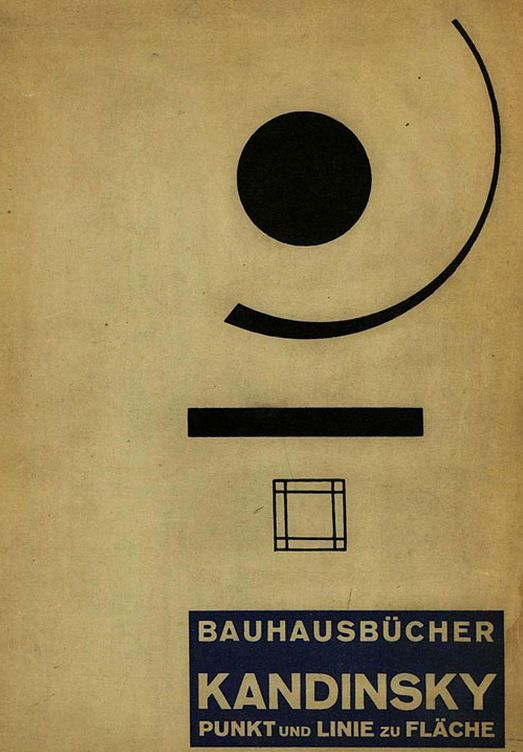
\includegraphics[width=0.70\textwidth]{img/PointAndLineToPlane.jpg}
	\caption[Point and Line to Plane]{Wassily Kandinsky - Point and Line to Plane}
	\label{fig:PointAndLineToPlane}
\end{figure}

The goal of this game is to obtain bigger territory than your opponent by drawing lines and overlapping these to create shapes.
The space is rotating slowly and this way it is possible to create all kinds of shapes.

\section{Game Mechanics}

The game can be played on both PC and iOS or Android devices.
For the PC version the field has to be tapped. The first tap, will mark the point to start the line from, pulling and letting go will create a line.
On Touchscreen devices two points have to be tapped at once to create a line.
Multiple lines can be drawn until a closed shape is produced.

The score depends on how much area the shape has. The player with the highest score wins.
The active players colour is green, other player is displayed in blue.

Players have a limited amount of ink that is displayed on the screen. The lower the ink meter gets, the faster it gets replenished. This increases the risk of being interrupted by the opponent when trying to create very great shapes, as this takes more time to do and forces you to wait, until you have enough ink.

The game is over when the set time of 30 seconds passes and the time runs out.
Since the space is rotating, it is necessary for the player to be quick, so they can create as big shapes as possible.

\section{The Development Team}

The tasks were distributed as follows:
\begin{center}
\begin{tabular}{r c l}
Kazuya Takahashi & Project Owner \\
                 & UI design \\
                 & Display Design of App \\
                 & Game Design \\
\hline
Alexander Johr   & Project Leader  \\
                 & Shaders \\
                 & Graphic Effects \\
                 & Gameplay Programming \\
								 & Audio Programming \\
\hline
Kousuke Kobayashi& Game Music  \\
\hline
Kyohei Takabe    & UI Programming  \\
\end{tabular}
\end{center}
\section{Gaining the Necessary Knowledge }


Two major subjects were needed to gain knowledge for: Networking for multiplayer and Shader programming for graphic effects.

For that the author of this documentation bought a bundle of video tutorials from udemy: ``Unity Networking From Scratch for (Unity 5 to Unity 2018+)'' and ``Shader Development from Scratch for Unity with Cg'' (Fig. \ref{fig:Tutorials}). The price of the bundle: 19.99 €. Both tutorials with a combined duration of 12 hours were completed to 100 \%.

\begin{figure}[htbp]
	\centering
		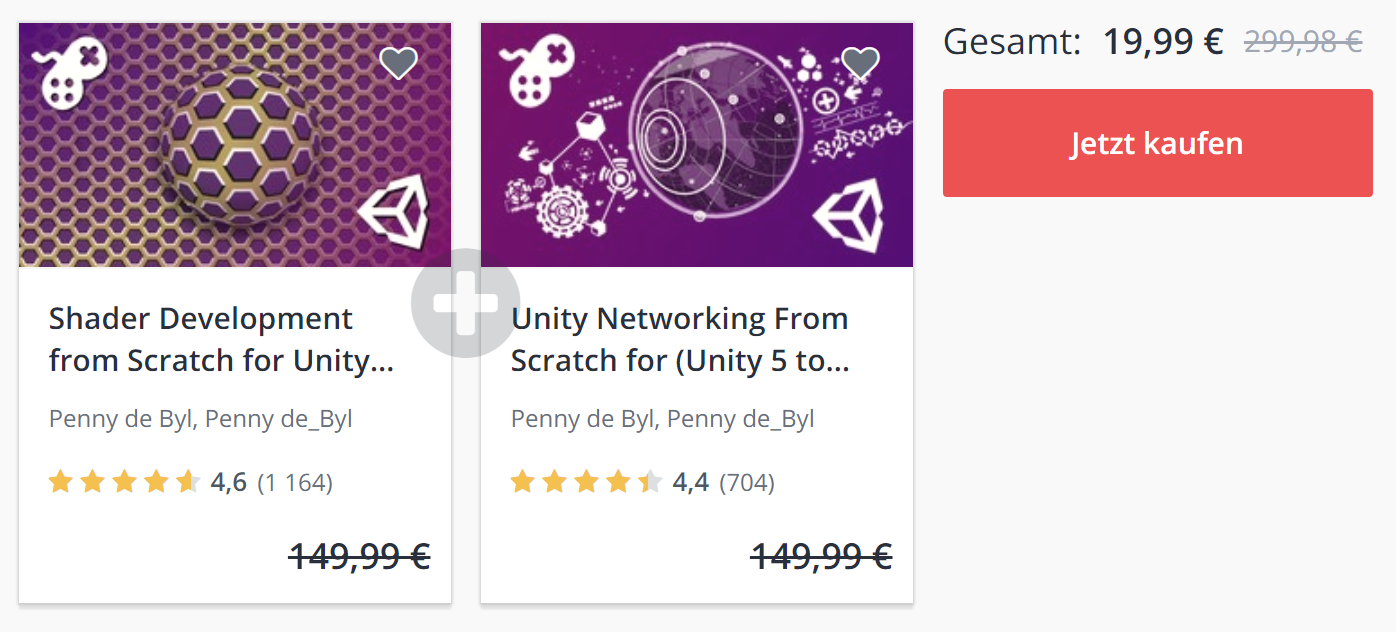
\includegraphics[width=1.00\textwidth]{img/Tutorials.png}
	\caption[Bought Udemy Tutorials]{Bought Udemy Tutorials}
	\label{fig:Tutorials}
\end{figure}

They were very useful for this project in the following features:

The networking tutorial taught
\begin{itemize}
	\item How to use the unity networking Lobby from the Asset store
	\item How to setup matchmaking with UNet
	\item How to send messages from one player to the other
\end{itemize}

The Shader tutorial taught
\begin{itemize}
	\item How to create shaders that render always even though they don’t face the camera. It was used for the shapes, that would not be visible anymore as the camera rotates around them. If that shader would not have been used, the shapes whould need to have twice the amount of vertices to be rendered from both directions.
	\item How to create Shaders that use the alpha channel. This allowed the lines to disappear with an animation where the lines gets faded out until it isn’t visible anymore.
	\item How to create a vertex shader that is used to create water waves. This shader was modified in order to give the lines a wiggly motion. That effect was used for lines, that get destroyed when they hit shapes and also when they cant placed because of insufficient ink or because there intersect with a shape before being placed
\end{itemize}

\section{Used Technologies}

Github was used as a way to share the game data and for version control.

The development was done in Unity3D.

The project management tool hacknplan was introduced to track the tasks. But apart from the project manager it was rarely used by the team and therefore soon abandoned.
Instead checklists were discussed in the Discord chart.

Discord was used for webcam-meeting sessions, for screen sharing and for regular chat.

The tool ScreenToGif was used by the author of this documentation to create status updates of the current game with gif animations.

Google Drive was used to share assets.

Google Docs was used to create drafts of the documentation.


\section{Challenges}

\subsection{Translation Challenges}

The team first used english as the language for chat messages and in the meetings.

Later the german project manager decided to translate every message into Japanese and back to English again to check if it was translated correctly (Fig. \ref{fig:Translation}).

\begin{figure}[htbp]
	\centering
		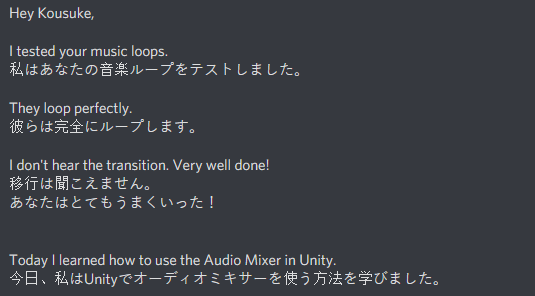
\includegraphics[width=1.00\textwidth]{img/Translation.png}
	\caption[Translation of every message into Japanese and back to English]{Translation of every message into Japanese and back to English}
	\label{fig:Translation}
\end{figure}

\subsection{Technical Challenges}

\subsubsection{Networking}

The programming of a multiplayer game proved to be a completely different thing, then programming a single player game.
The first approach to add the network functionality to the singleplayer game failed. Instead the game had to be programmed from scratch again.

It is important to keep in mind, that almost every action that the player does has to be send to the opponent.

That means that the client has to inform the server each time:
\begin{itemize}
	\item a line is created,
	\item a line is updated,
	\item a line is deleted,
	\item a shape is created and
	\item the game ends.
\end{itemize}

Then the server needs to inform the all clients about that update. The Server can’t decide which client he sends the update to, instead he informs all clients. THat means that even the client that send the message received that message again. The clients needs to check if the message was sent by the opponent.

Each player has to memorize its own lines and shapes as well as the opponents lines and shapes. The client also can’t reference the game objects directly by a C\# Reference. Instead each line and shape needs an id to be found on the client.

\subsubsection{Creating Shapes from Lines}


Constructing the shapes from the given points and lines has posed some difficulties. 
The assumption was, that this Jarvis-March algorithm would connect the points formed by the crossing lines. The algorithm is also called ``Gift Wrapping Algorithm'' because it is calculating the convex hull of the shape.

\begin{figure}[htbp]
	\centering
		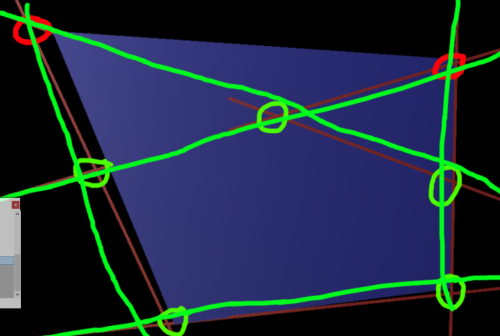
\includegraphics[width=0.70\textwidth]{img/ConnectLinesToShape.png}
	\caption[Gift wrapping algorithm does not fit]{Gift wrapping algorithm does not fit}
	\label{fig:ConnectLinesToShape}
\end{figure}

Unfortunately this meant, that points, that formed outside of the wrapper-like outline, weren’t counted and ignored. Therefore more area would be scored than should be going by the lines drawn. The Gift Wrapping Algorithm connects the the points on the top which are outlined in red (Fig. \ref{fig:ConnectLinesToShape}). However, the shape should be formed by the green lines instead. The two red points are connected in the resulting shape, but there isn’t a green line connecting them.



A different approach and custom algorithm was needed to connect the lines into a shape. For that every point memorized its two intersecting lines. Then it is checked if one line is memorized by two different intersections. If two intersection points have a line in common, they get connected. This results in multiple possible shapes, because a set of lines can form multiple connections. In the right figure for example the two nested triangles on top are also counted as shapes. The algorithm then finds the shape, that has the most intersections, which is the biggest shape and contains als the nested shapes, which need to be ignored.


\subsubsection{Effect for Faulty Line Placement}
A wiggly motion was implemented for the lines (Fig. \ref{fig:Wiggle1}), when it’s impossible to place a line.

\begin{figure}[htbp]
	\centering
		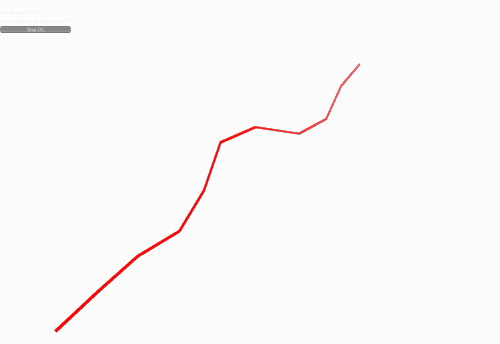
\includegraphics[width=0.50\textwidth]{img/Wiggle1.png}
	\caption[Line with wiggly motion faces the camera]{Line with wiggly motion faces the camera}
	\label{fig:Wiggle1}
\end{figure}

A plane was used for this, but the issue with it was, that the line wasn’t visible when the edge was turned toward but none of the faces are pointed to the camera (Fig. \ref{fig:Wiggle2}).

\begin{figure}[htbp]
	\centering
		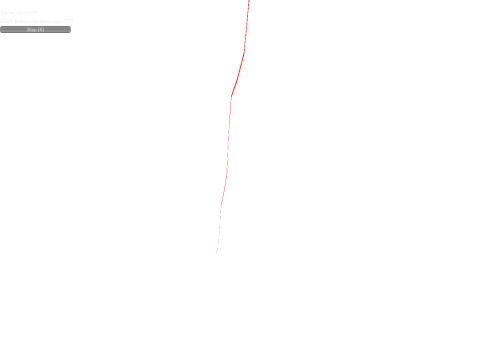
\includegraphics[width=0.50\textwidth]{img/Wiggle2.png}
	\caption[Line with wiggly motion does not face the camera]{Line with wiggly motion does not face the camera}
	\label{fig:Wiggle2}
\end{figure}

To get the line to be visible again the rotation would need to be adjusted. This can unfortunately not be achieved by simply changing the LookRotation towards the camera.






To solve this the following solution has been implemented:
The needed normal is the one that points the most directly toward the camera.
It is not possible to find it just like that. First the point has to be found at which the right normal hits the camera.
This can be calculated mathematically.
Now the point can be found at which the normal would have to be to point toward the camera.
For this the position of the camera is projected onto the lines vector (Fig. \ref{fig:Projection}).
\begin{figure}[htbp]
	\centering
		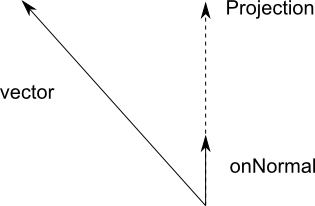
\includegraphics[width=0.50\textwidth]{img/Projection.jpg}
	\caption[Projection of a Vector]{Projection of a Vector}
	\label{fig:Projection}
\end{figure}
Going from this projectionpoint, it is possible to calculate the vector, which points at the camera. This is done by:
camera position - projection point
This vector is the so called “Forward Vector”. Afterwards it is necessary to figure out which one is the “Up-Vector” of the planes look rotation. This is done by:
endpoint - startpoint
With the help of the Unity function Quaternion.LookRotation(Vector3 forward, Vector3 up) the correct rotation for the plane can be calculated and the line is visible from all viewpoints.

\section{Project Diary}

\subsection{22.10.2018 - First Meeting}

The project seemed to have started very well. Alexander Johr prepared a mockup of an iPad. With that and an underling blank paper he tried to describe what he understood from the game idea. He did it in order to avoid any misunderstandings. He assumed that the team members would disagree with his explanation if he misinterpreted something. The team members agreed that everything is correct. Alexander Johr assumed that the game would be a single player game. It was until very late in in the project on 26.11.2018 that one team member shared, that he thought the game should be a multiplayer game.

\begin{figure}[htbp]
	\centering
		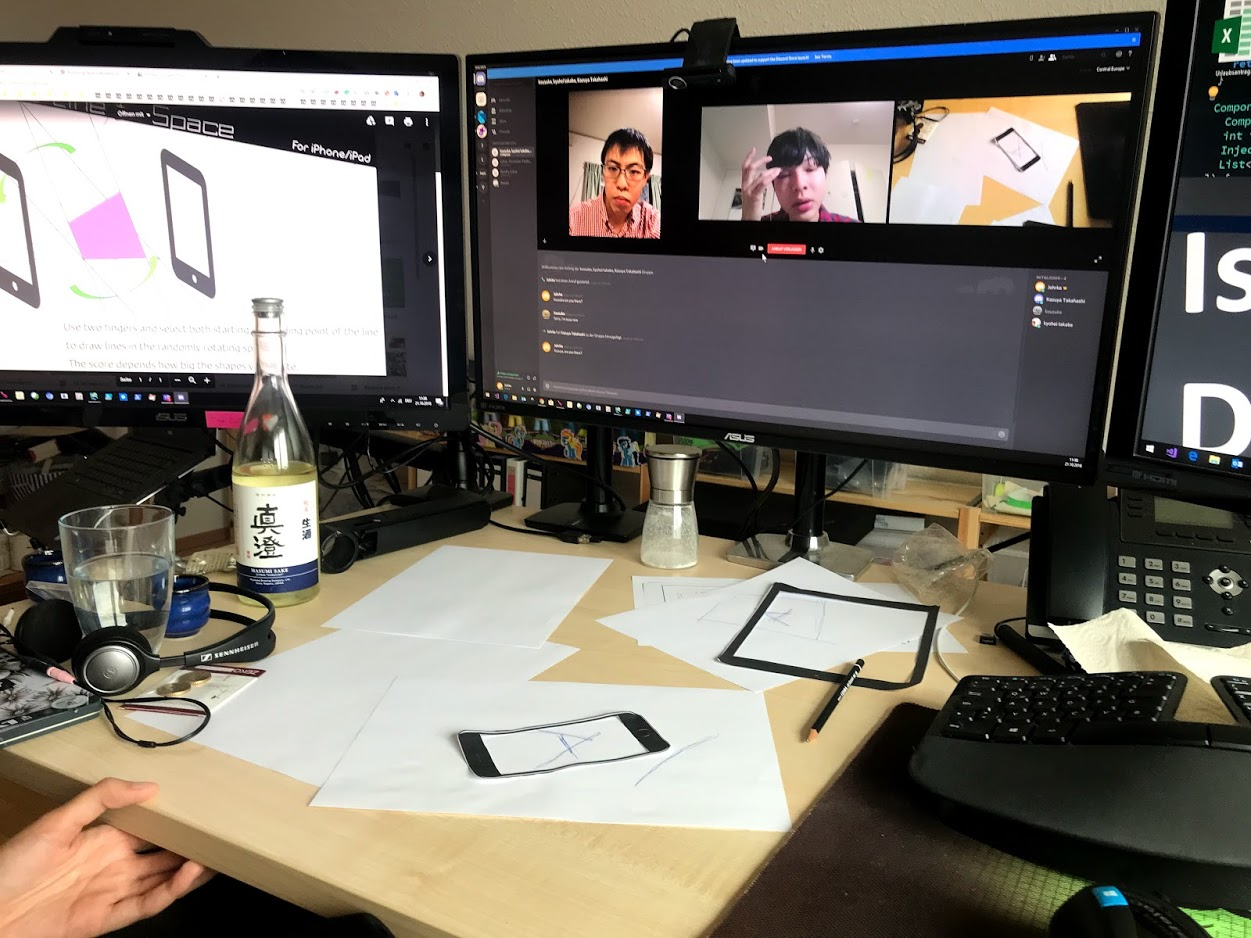
\includegraphics[width=1.00\textwidth]{img/FirstMeeting1.png}
	\caption[First Meeting]{First Meeting}
	\label{fig:PointAndLineToPlane}
\end{figure}

\begin{figure}[htbp]
	\centering
		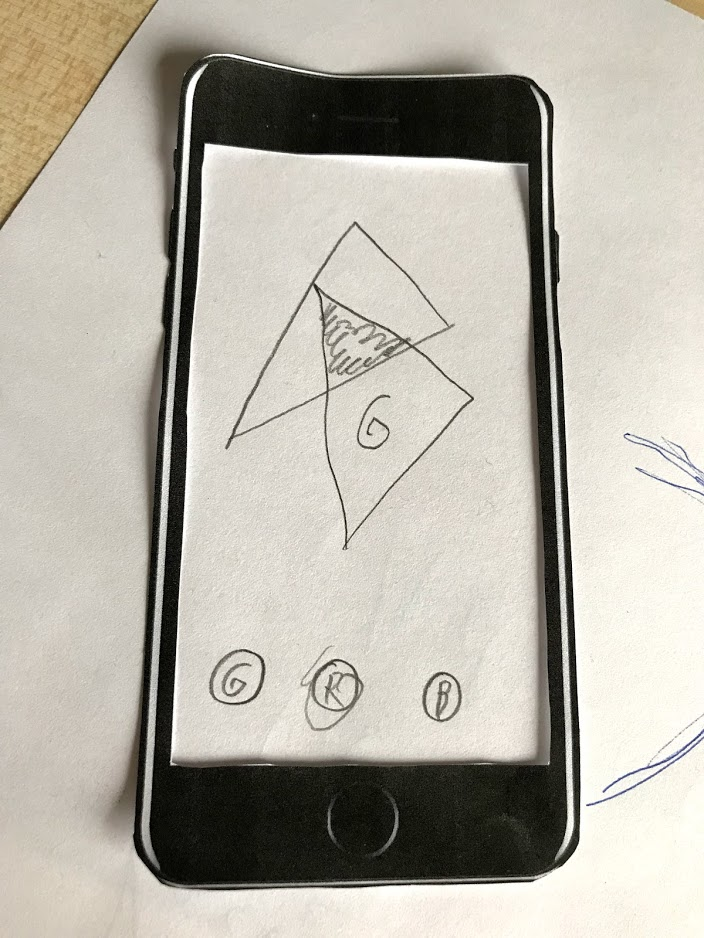
\includegraphics[width=1.00\textwidth]{img/FirstMeeting2.png}
	\caption[First Meeting - Mockup]{First Meeting - Mockup}
	\label{fig:PointAndLineToPlane}
\end{figure}

It was also decided which tasks should be done by which team member:

\begin{itemize}
	\item Alexander Johr: Shaders, Graphic effects, (If required I could also code)
	\item Kazuya Takahashi: UI, Menu, Display design of the app (2D), Game design(basic concept), Advertisement
	\item Kousuke Kobayashi: Music and Sound Effects
	\item Kyohei Takabe: Programming, 3d modelling (optional)
\end{itemize}

\subsection{26.10.2018 - Second Meeting}
Alexander Johr showed the game sinuous game  http://www.sinuousgame.com in order to:
\begin{itemize}
	\item Show how a game can use multiple music tracks that play in parallel. The game can fade from one track to another if the context of the game changes. Start Screen: calm music; play screen: additional sound effects added to the game; invincibility upgrade gained: fast exaggerated music

	\item Show a game with very simplistic shapes
\end{itemize}

Kousuke Kobayashi shared his first version of the game music loop. (Assets/Point and Lines to Space01.wav)

Alexander Johr created the github repository: https://github.com/AlexanderJohr/point-and-line-to-space.git

Kyohei Takabe and Alexander Johr both agreed, that Alexander Johr should programm the first playable, as he has more knowledge with unity. After the first playable works, he would hand over the gameplay programming to Kyohei and focus again on graphics effects.

\subsection{29.10.2018 - Third Meeting}
All team members were invited to the github repository.

Alexander Johr finished the first playable and showed it to the team. The first playable allowed to create triangles only. It cost 11 hours to create that first playable.

\subsection{31.10.2018 - Fourth Meeting}

Alexander Johr introduced tutorials on how to use unity remote for android and ios devices. He tasked every team member to study the tutorial for the device they possess in order to test the game frequently.

\subsection{02.11.2018 - Fifth Meeting}
Alexander Johr explained the code of the first playable to Kyohei Takabe.

Alexander Johr shared the information he gained from his professor Prof. Dominik Wilhelm. He explained the importance of the title screen. It is the title screen that is remembered. If the player doesn’t understand the game then the title screen was the only thing, that he saw. If that screen is not great, then this is the only thing that the player remembers of that game.

Also Prof. Dominik Wilhelm shared various ideas of different look and feel like basic Bauhaus Design (Fig. \ref{fig:Bauhaus}) or the look and feel of the games Vib Ribbon (Fig. \ref{fig:VibRibbon}), Rez Infinite (Fig. \ref{fig:RezInfinite}) and Geometry Wars (Fig. \ref{fig:GeometryWars}).

\begin{figure}[htbp]
	\centering
		
\includegraphics[width=0.40\textwidth]{img/Bauhaus.jpg}
	\caption[Basic Bauhaus Design]{Basic Bauhaus Design}
	\label{fig:Bauhaus}
\end{figure}
\begin{figure}[htbp]
	\centering
		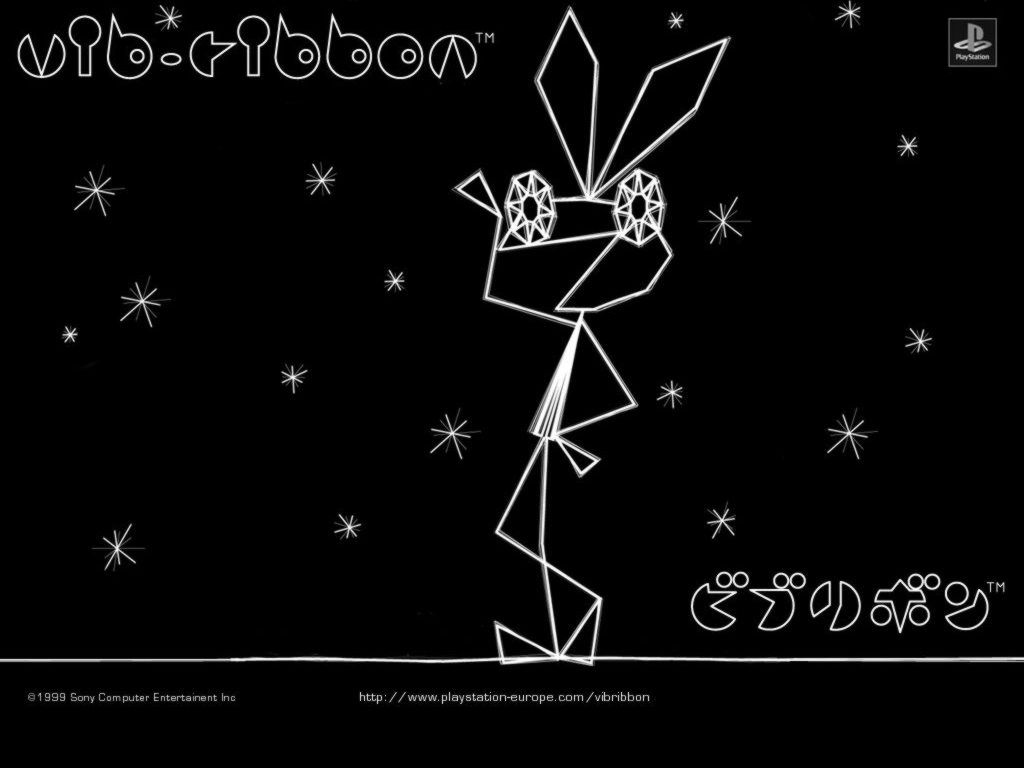
\includegraphics[width=0.40\textwidth]{img/VibRibbon.jpg}
	\caption[Look and Feel of the Game Vib Ribbon]{Look and Feel of the Game Vib Ribbon}
	\label{fig:VibRibbon}
\end{figure}
\begin{figure}[htbp]
	\centering
		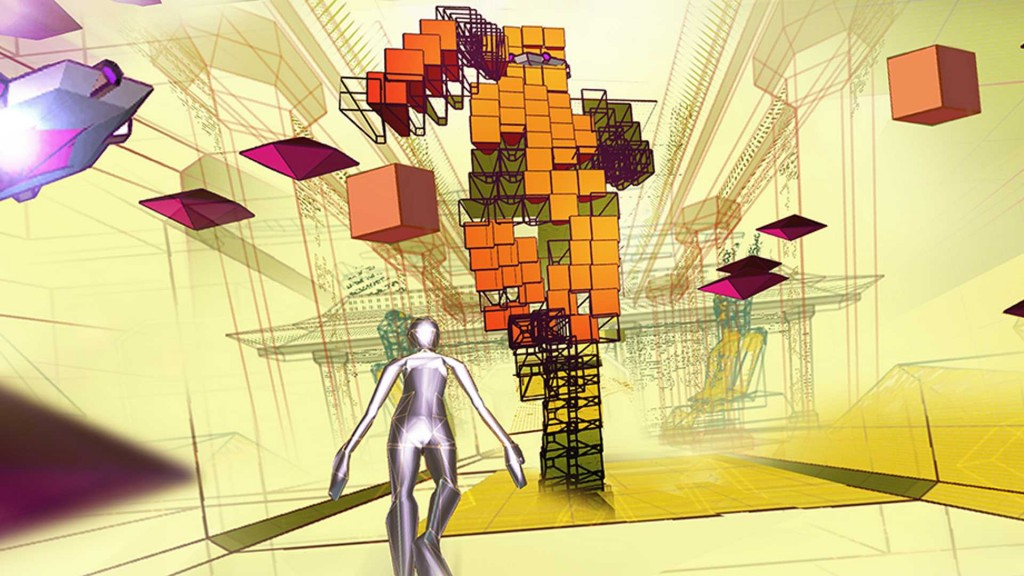
\includegraphics[width=0.40\textwidth]{img/RezInfinite.jpg}
	\caption[Look and Feel of the Game Rez Infinite]{Look and Feel of the Game Rez Infinite}
	\label{fig:RezInfinite}
\end{figure}
\begin{figure}[htbp]
	\centering
		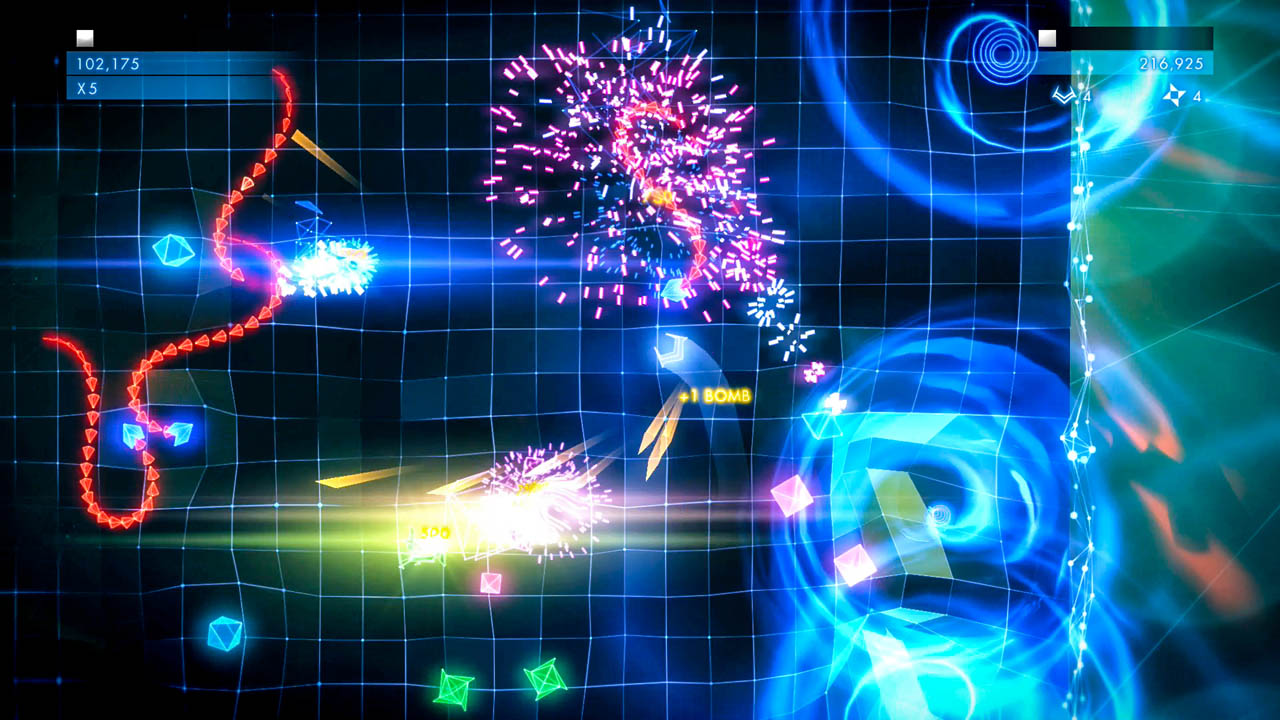
\includegraphics[width=0.40\textwidth]{img/GeometryWars.jpg}
	\caption[Look and Feel of the Game Geometry Wars]{Look and Feel of the Game GeometryWars}
	\label{fig:GeometryWars}
\end{figure}

As the skill matrix showed that Kazuya Takahashi has the most experience in 2D Art it was decided that he should work on the title screen.

Kazuya Takahashi explained the idea, that the background music of the game could change, when the time runs out, just as in super mario games. Alexander Johr introduced the team to the tool Fmod which could be used for that.


\subsection{05.11.2018  - Sixth Meeting}
Kousuke Kobayashi provided his second version of the background music. (Assets/Point and Lines to Space02.wav)


\subsection{17.11.2018 - Seventh Meeting}
Alexander Johr explained Kyohei Takabe how properties work in C\#.

Kyohei Takabe showed what he learned from the Unity tutorial he made  (Fig. \ref{fig:UnityTutorial}). Kyohei Takabe also showed what he learned from his books on git versioning.

\begin{figure}[htbp]
	\centering
		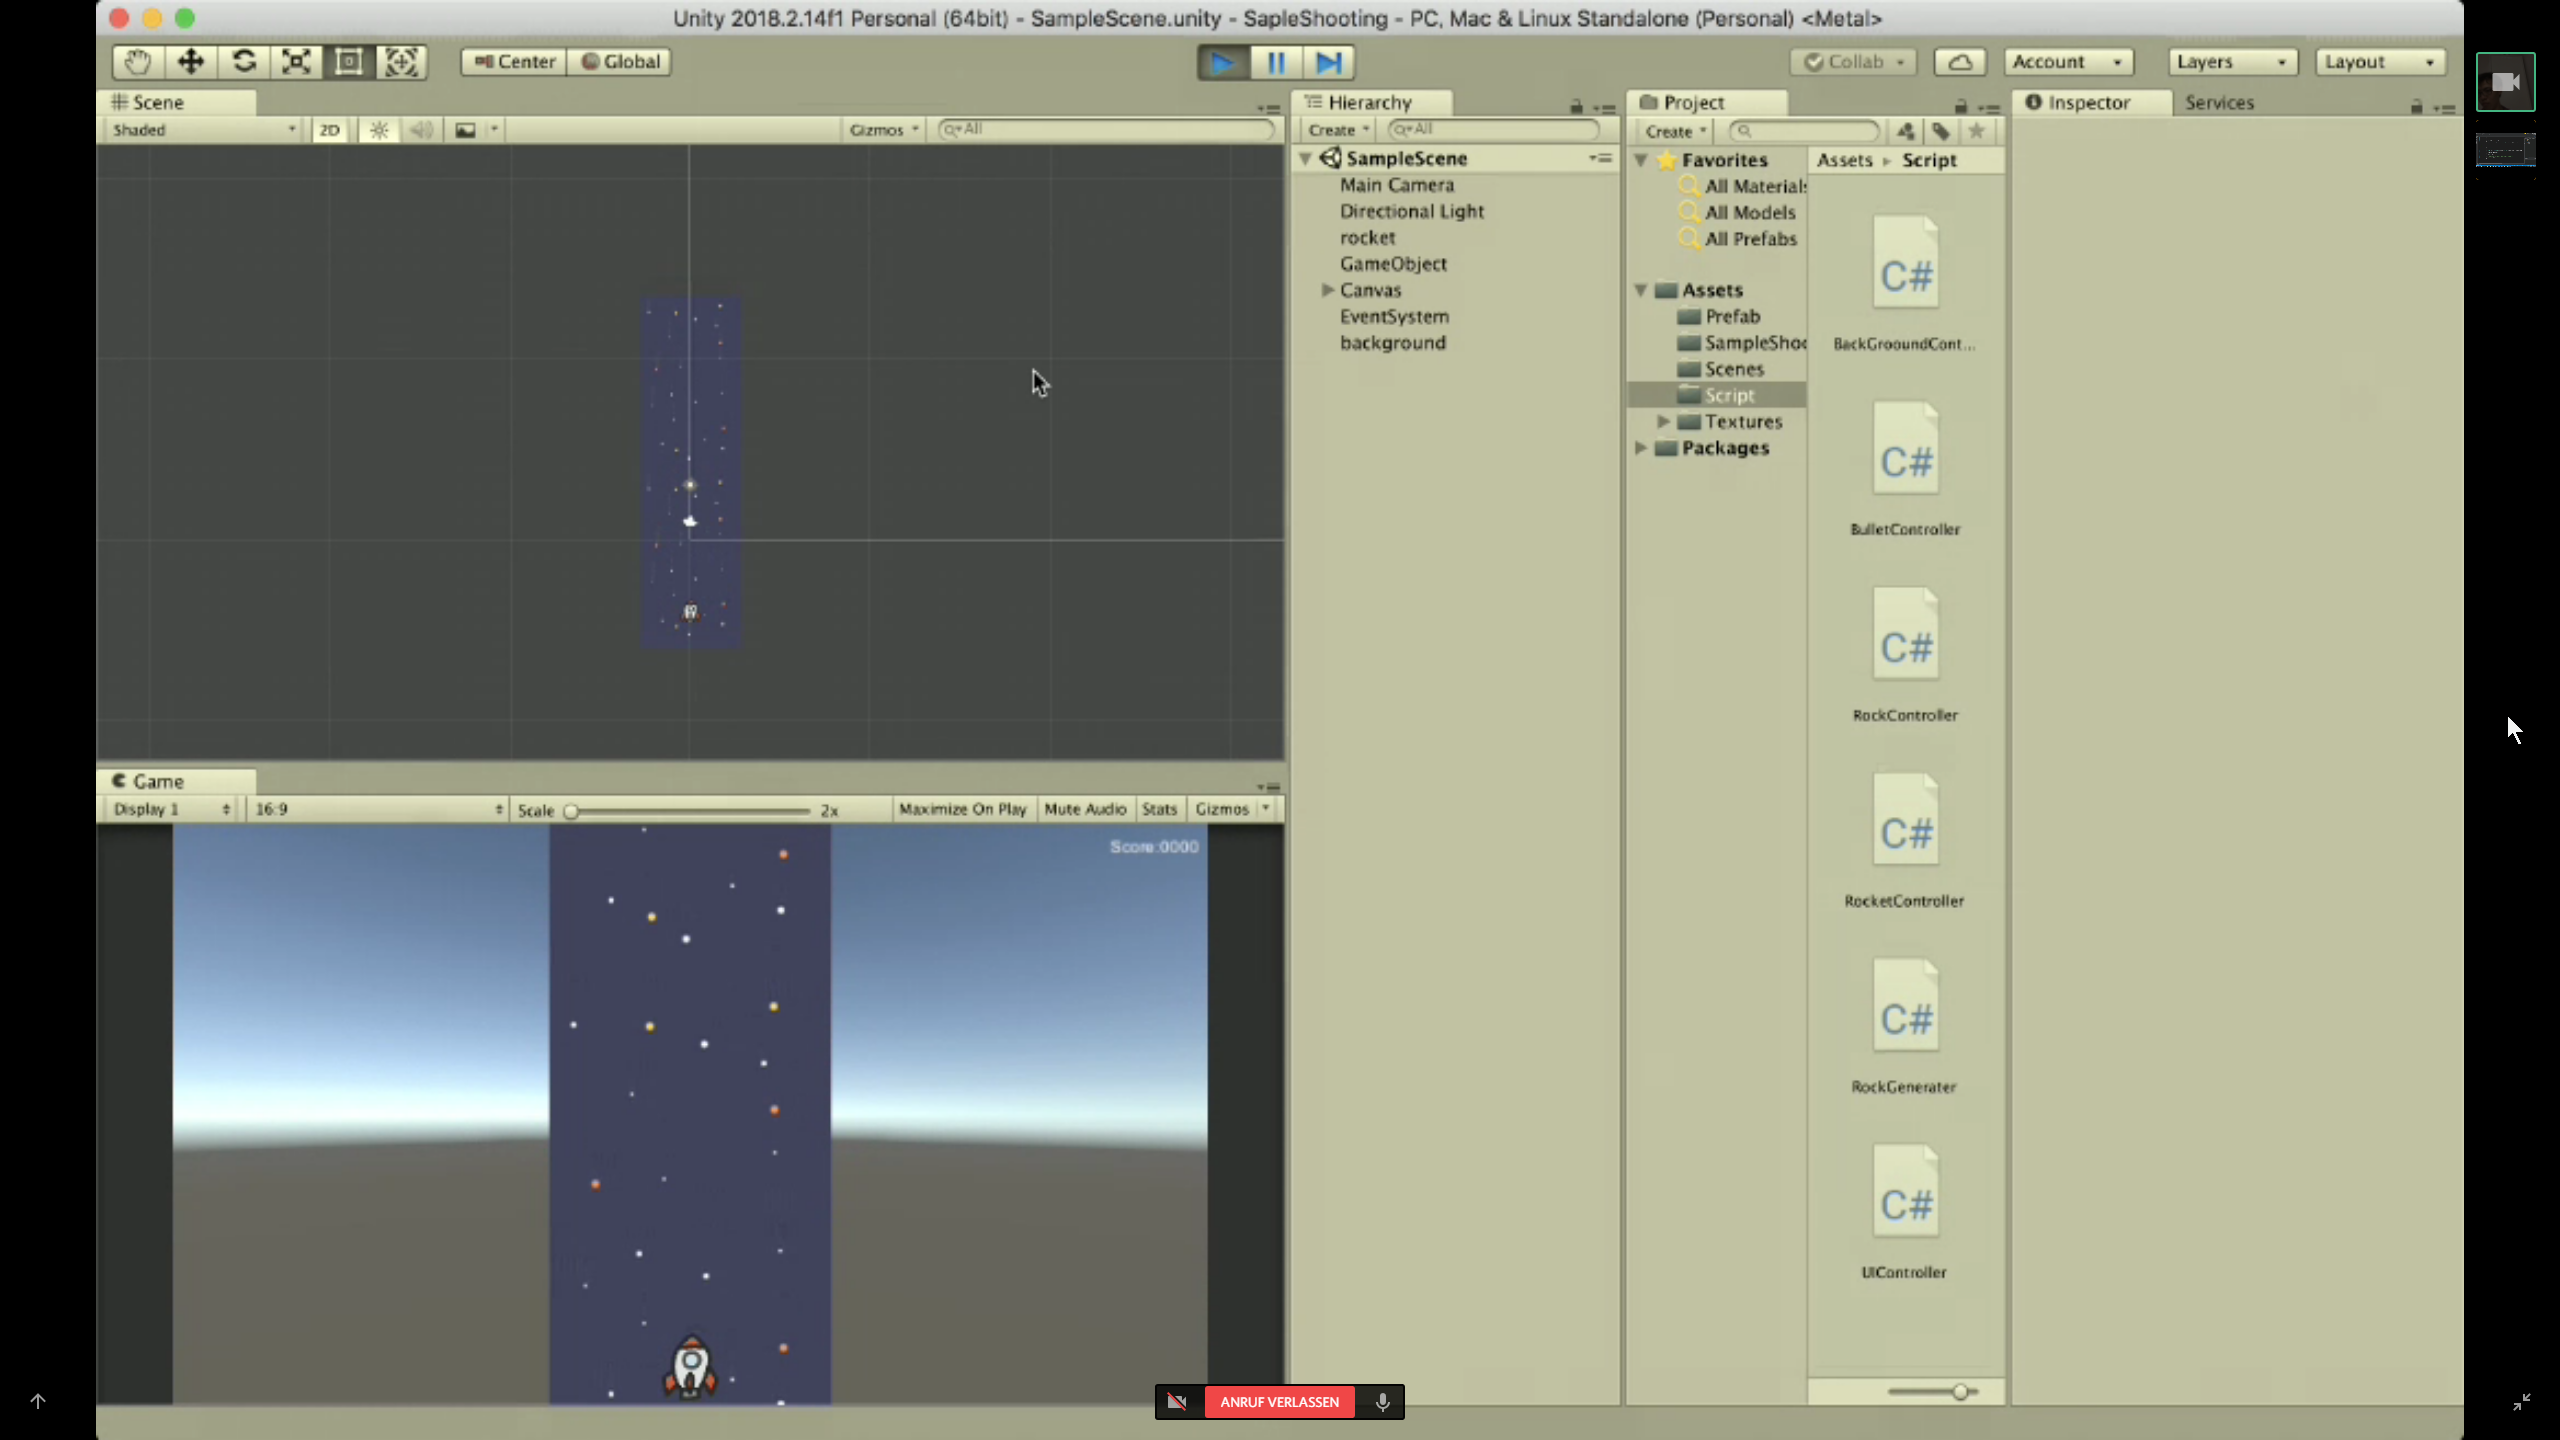
\includegraphics[width=1.00\textwidth]{img/UnityTutorial.png}
	\caption[Unity Tutorial for a 2D Game]{Unity Tutorial for a 2D Game}
	\label{fig:UnityTutorial}
\end{figure}

Alexander Johr shared his experience with the Graham scan algorithm and that turned out not to be usable for the project.

Kyohei Takabe was tasked to create the UI for the game using placeholders.


\subsection{18.11.2018 - Eighth Meeting}
Alexander Johr explained to Kyohei Takabe how git fork and git pull requests work


\subsection{19.11.2018 - Ninth Meeting}
Kousuke Kobayashi decided to learn how include sound into unity games and learn C\# in order to manipulate them.

Alexander Johr shared the example that Prof. Dominik Wilhelm provided to him on how the music could sound like: Luigi Russolo and the Futurista Sound System - https://www.youtube.com/watch?v=VHhzC9bXp4E 

Alexander Johr showed Kousuke Kobayashi and Kazuya Takahashi the basics on how to include music into Unity.

Alexander Johr showed what the tool Fmod offers Unity Developers (Fig. \ref{fig:fmod}).

\begin{figure}[htbp]
	\centering
		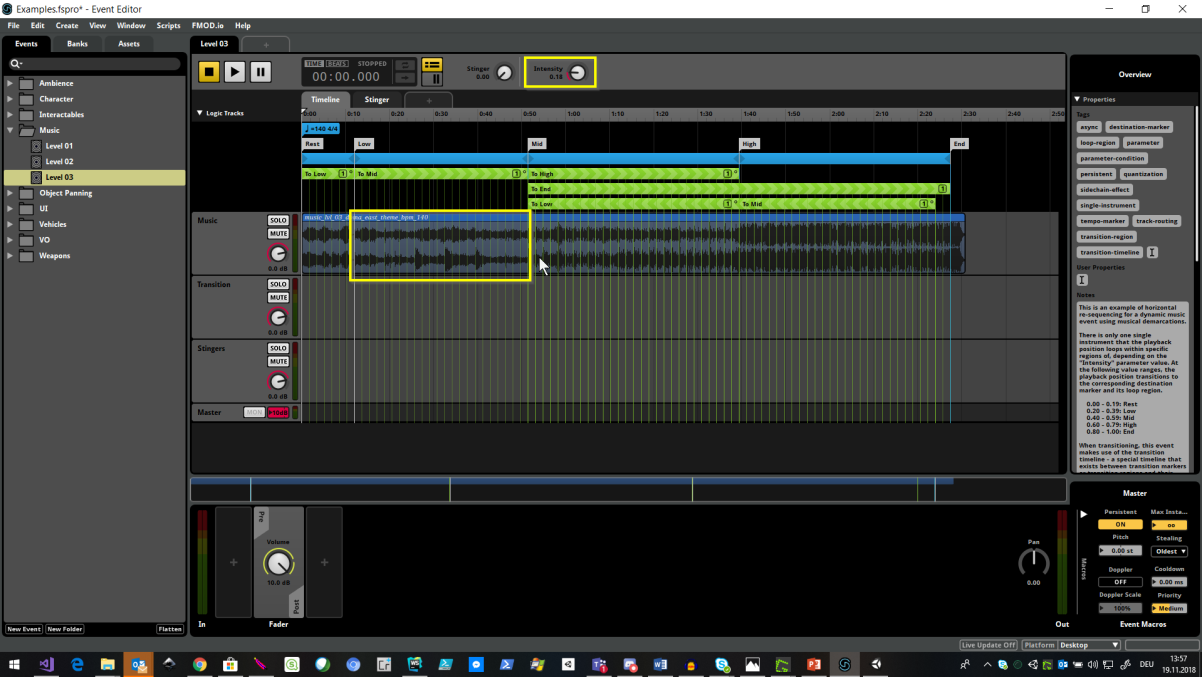
\includegraphics[width=1.00\textwidth]{img/fmod.png}
	\caption[Fmod]{Fmod}
	\label{fig:fmod}
\end{figure}

\subsection{22.11.2018 - Tenth Meeting}
Kyohei Takabe informed the team that he finished the UI prototype with placeholders.


\subsection{26.11.2018 - Eleventh Meeting}
Kousuke Kobayashi provided sound effects for creating shapes.

It was decided, that the game should support landscape mode. Portrait mode is optional.

Alexander Johr showed that the game now supports to create shapes with more than 3 edges. He also explained that the next step would be to introduce enemies into the game.

Kousuke Kobayashi asked what is meant by ‘enemies’ because he thought the game would be a multiplayer game. Kazuya Takahashi agreed that the first idea of the game was a multiplayer game. It was later discussed how the misunderstanding came to be. When the Alexander Johr described what he understood from the game idea in the first meeting, the team didn’t interrupt him, as he assumed the game would be a singleplayer game. Instead they assumed that the conveyed information is what Alexander Johr thinks of what would be technically possible.

That teached the team to never assume anything!

Kazuya Takahashi showed his drafts for the splash and Menu Screen to the team (Fig. \ref{fig:Menu4}, \ref{fig:Menu5}, \ref{fig:Menu1}, \ref{fig:Menu2}, \ref{fig:Menu3} ).

\begin{figure}[htbp]
	\centering
		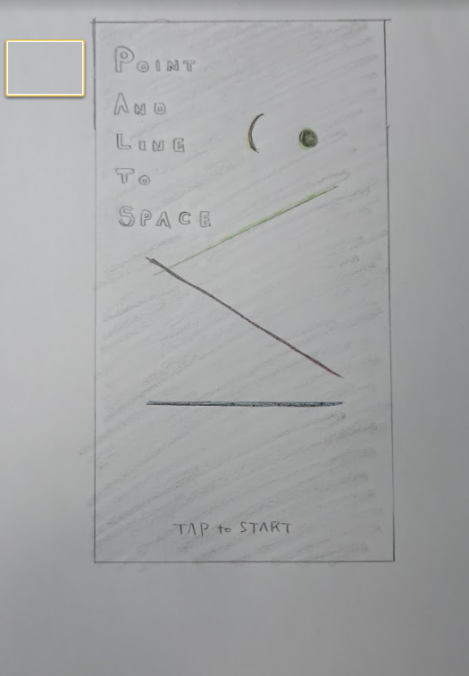
\includegraphics[width=1.00\textwidth]{img/Menu4.png}
	\caption[Splash Screen Draft 1]{Splash Screen Draft 1}
	\label{fig:Menu4}
\end{figure}
\begin{figure}[htbp]
	\centering
		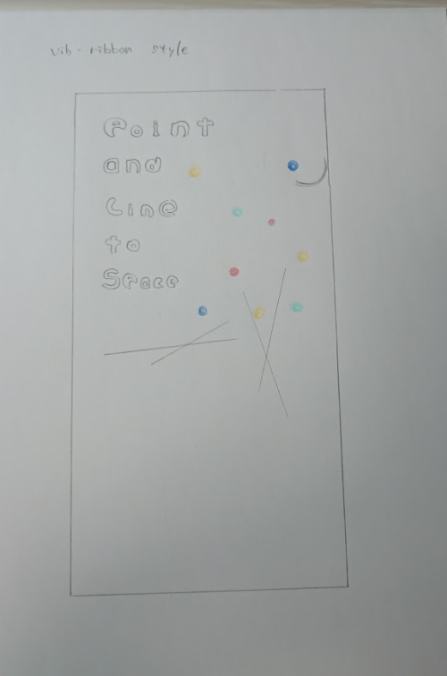
\includegraphics[width=1.00\textwidth]{img/Menu5.png}
	\caption[Splash Screen Draft 2]{Splash Screen Draft 2}
	\label{fig:Menu5}
\end{figure}

\begin{figure}[htbp]
	\centering
		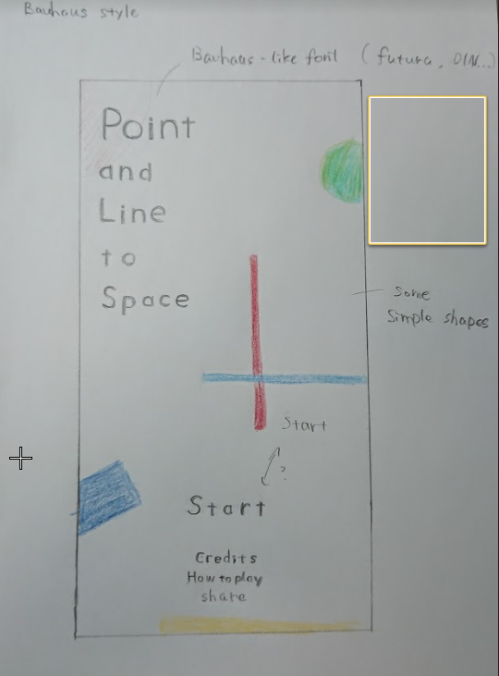
\includegraphics[width=1.00\textwidth]{img/Menu1.png}
	\caption[Menu Screen Draft 1]{Menu Screen Draft 1}
	\label{fig:Menu1}
\end{figure}
\begin{figure}[htbp]
	\centering
		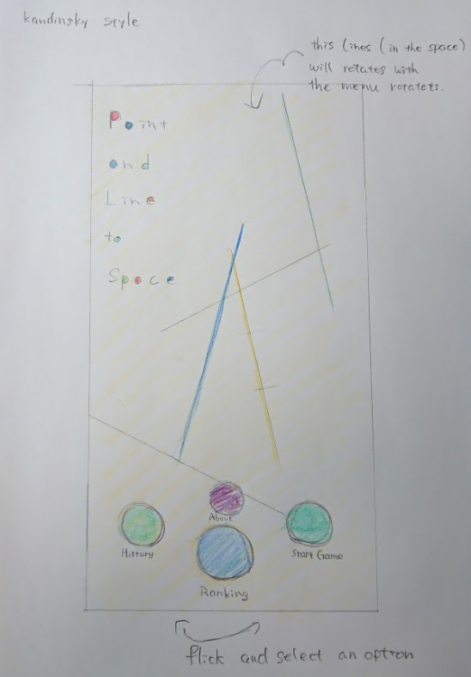
\includegraphics[width=1.00\textwidth]{img/Menu2.png}
	\caption[Menu Screen Draft 2]{Menu Screen Draft 2}
	\label{fig:Menu2}
\end{figure}
\begin{figure}[htbp]
	\centering
		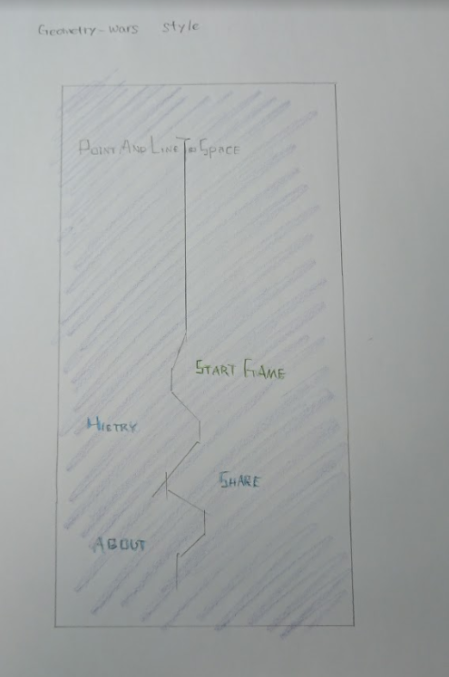
\includegraphics[width=1.00\textwidth]{img/Menu3.png}
	\caption[Menu Screen Draft 3]{Menu Screen Draft 3}
	\label{fig:Menu3}
\end{figure}


\subsection{17.12.2018 - Twelfth Meeting}
Alexander Johr informed the team that he completed the Networking tutorial and he will start creating the game from ground up, this time as a multiplayer game. The rest of the team was tasked to create the final splash screen and menu screen.



\subsection{20.01.2019 - Thirteenth Meeting}
Kazuya Takahashi provided UI drafts for the final splash screen and menu screen (Fig. \ref{fig:splash1}, \ref{fig:splash2}).

\begin{figure}[htbp]
	\centering
		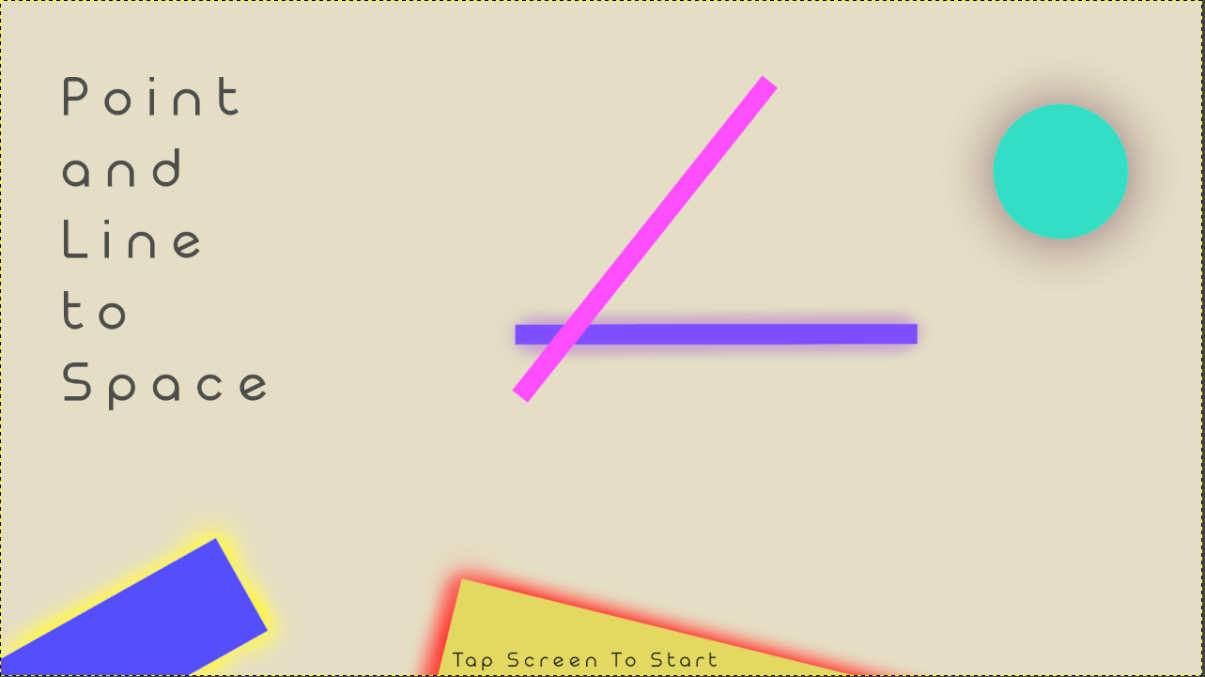
\includegraphics[width=1.00\textwidth]{img/splash1.png}
	\caption[Splash Screen Draft 3]{Splash Screen Draft 3}
	\label{fig:splash1}
\end{figure}

\begin{figure}[htbp]
	\centering
		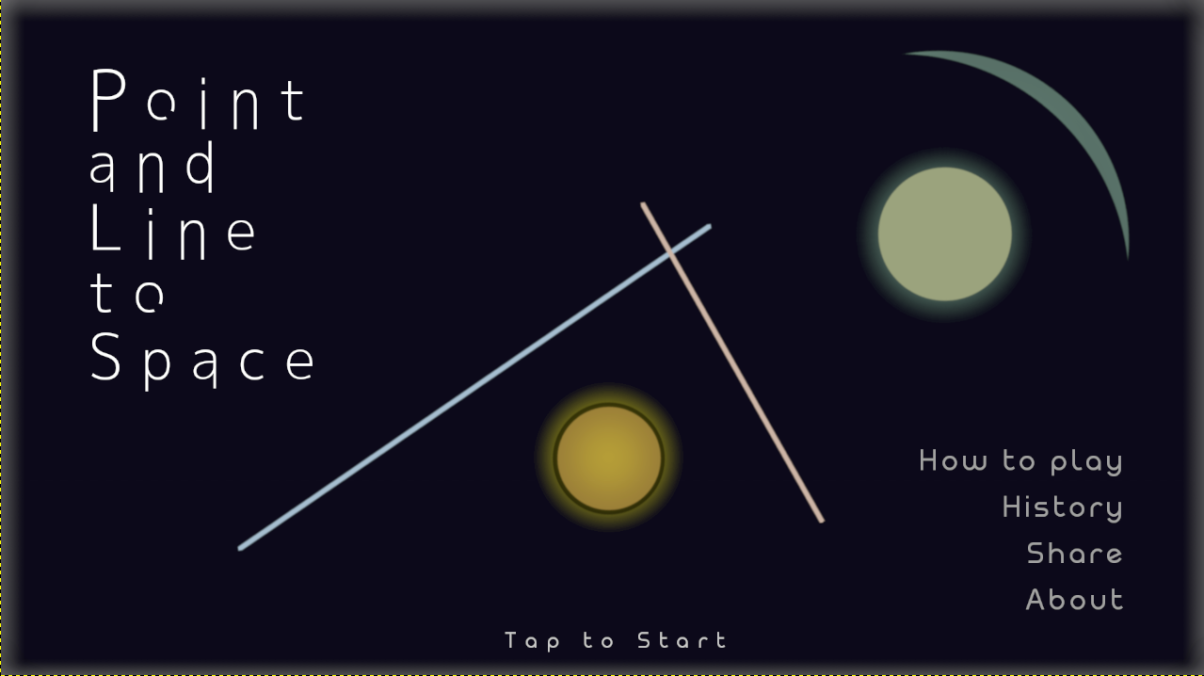
\includegraphics[width=1.00\textwidth]{img/splash2.png}
	\caption[Menu Screen Draft 4]{Menu Screen Draft 4}
	\label{fig:splash2}
\end{figure}

\subsection{03.02.2019  - Fourteenth Meeting}
Kyohei Takabe transferring the final UI into unity. But it turned out, that it doesn’t respond to different screen sizes and only works on the iPhone that it was tested on (Fig. \ref{fig:UiInUnity1}). 

\begin{figure}[htbp]
	\centering
		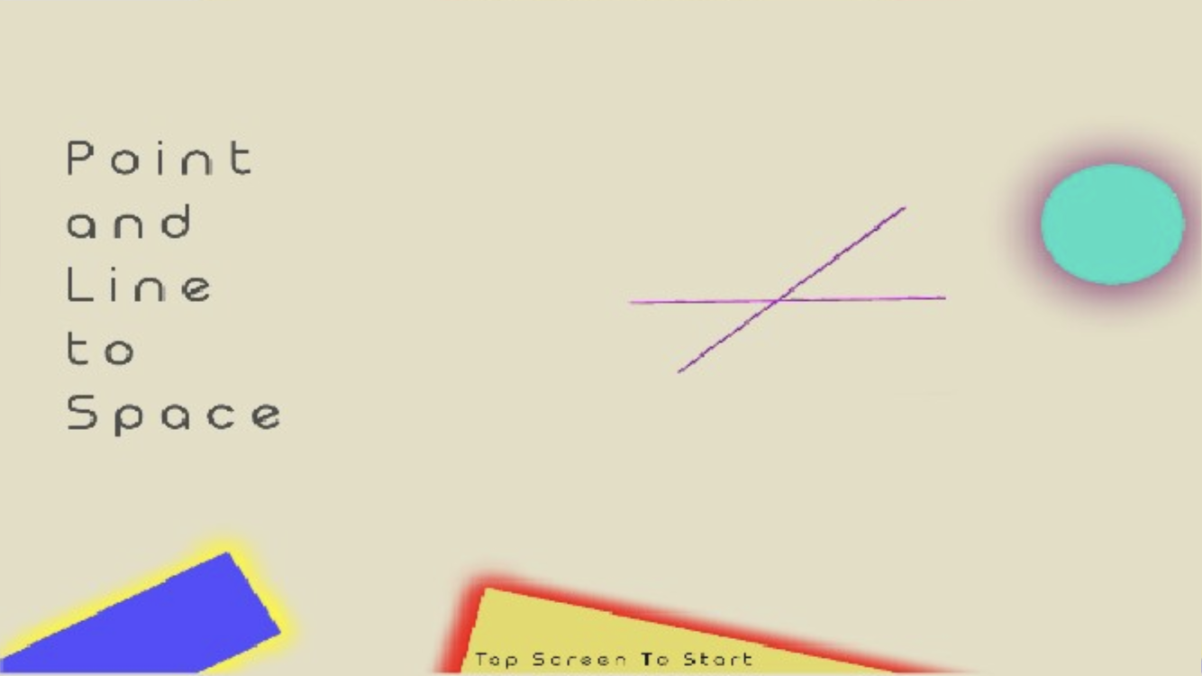
\includegraphics[width=1.00\textwidth]{img/UiInUnity1.png}
	\caption[UI Transfered into Unity]{UI Transfered into Unity}
	\label{fig:UiInUnity1}
\end{figure}

Kousuke Kobayashi provided further sound effects for creating the lines.

The whole team was tasked to create documentation on the things that they worked on.


\subsection{07.02.2019  - Fifteenth Meeting}
Alexander Johr informed the team that he completed the the network functionality for the game including a network lobby to create matches.

Kousuke Kobayashi provided five background music tracks that are loopable and can be used for different contexts in the game. (Assets/Music Loops)

Alexander Johr described how the splash and menu screen need to be created.

\subsection{09.02.2019  - Sixteenth Meeting}
Alexander Johr informed the team that he completed wiggly motion effect for the lines that can’t be placed.


\subsection{11.02.2019  - Seventeenth Meeting}
Kyohei Takabe finished the splash and menu screen that is functional on different devices with different resolutions.

Kazuya Takahashi provided UI drafts for the play screen (Fig. \ref{fig:PlayScreen1}) and the result screen (Fig. \ref{fig:ResultDraft1}).

\begin{figure}[htbp]
	\centering
		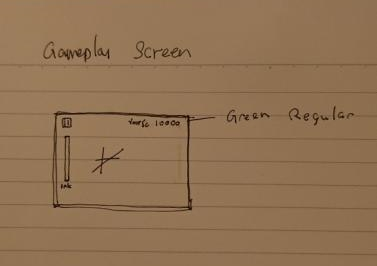
\includegraphics[width=1.00\textwidth]{img/PlayScreen1.jpg}
	\caption[Play Screen Draft]{Play Screen Draft}
	\label{fig:PlayScreen1}
\end{figure}

\begin{figure}[htbp]
	\centering
		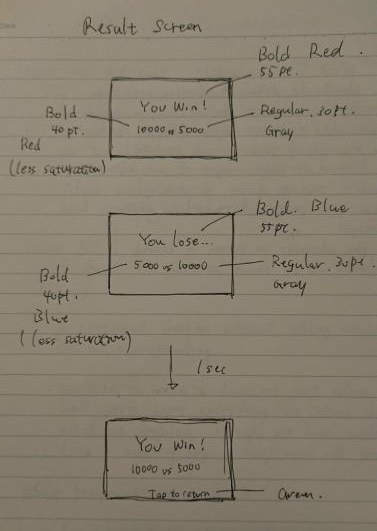
\includegraphics[width=1.00\textwidth]{img/ResultDraft1.jpg}
	\caption[Result Screen Draft]{Result Screen Draft}
	\label{fig:ResultDraft1}
\end{figure}
 
\end{document}